\documentclass{beamer}
\usepackage{HECbeamer}
% \usepackage{pgfpages}
% \pgfpagesuselayout{4 on 1}[letterpaper, landscape, border shrink=5mm]
\title[\color{white}{MATH 60604A \S~5e - $\mathsf{AR}(1)$ covariance model}]{\texorpdfstring{MATH 60604A \\Statistical modelling \\ \S~5e - Covariance models: first-order autoregressive covariance}{MATH 60604A \\Statistical modelling \\ \S~5e - Covariance models: $\mathsf{AR}(1)$}}
\author{Léo Belzile}
\institute{HEC Montréal\\
Department of Decision Sciences}
\date{} 

\begin{document}
\frame{\titlepage}

\begin{frame}
\frametitle{Alternative covariance structure}
\bi
\item We saw how to model the correlation between repeated measures from the same person, while assuming a compound symmetry structure. 
\item This structure was certainly plausible, since the parameter estimating within-person correlation was significantly different from zero. 
\item But how do we know if this is the best correlation structure? There may be another more appropriate structure for the correlation.
\item There are several other covariance structures; in fact, \SASlang{} has a large number of possibilities. We will show several here; an exhaustive list can be found within \SASlang{}.
\ei
\end{frame}

\begin{frame}
\frametitle{Choosing the covariance structure}
\bi
\item In many cases, the correlation structure is considered to be a nuisance parameter. More precisely, usually the primary interest in a study is the effect of the predictor variables, $\bs{\beta}$. 
\item In this case, the covariance structure is not particularly interesting, other than the fact that  we need to account for correlation to make sure our inference concerning $\bs{\beta}$ is valid. 
\item We could base the choice of covariance structure on information criteria if the models are not nested (provided they have the same covariates if the model is fitted using REML).
\ei
\end{frame}

\begin{frame}
\frametitle{Auto-regressive structure}
\bi
\item The compound symmetry structure used before assumes the correlation between two observations is always the same. 
\item When we have repeated measures taken at different time points, as we do here, 
it's possible that the magnitude of the correlation depends on the amount of time between observations. 
\item We might believe that the closer together observations
are in time, the more they are correlated. The \alert{autoregressive of order 1}, or \alert{$\mathsf{AR}(1)$}, structure allows us to do this.
\item The $\mathsf{AR}(1)$ model has two parameters: a correlation parameter $\rho$ and a variance parameter $\sigma^2$.
\ei
\end{frame}

\begin{frame}
\frametitle{Auto-regressive structure}
\bi
\item For subject $i$ with five repeated measurements, 
the correlation matrix is 
\[
\mathbf{R}_i=
  \begin{pmatrix}
   1 & \rho & \rho^2 & \rho^3 & \rho^4\\
    \rho & 1 & \rho & \rho^2 & \rho^3\\
    \rho^2 & \rho & 1 & \rho &  \rho^2\\
       \rho^3 & \rho^2 & \rho & 1 & \rho\\
       \rho^4 & \rho^3 & \rho^2 & \rho & 1
  \end{pmatrix}.
\]
\item The covariance structure is 
\begin{align*}
\bs{\Sigma}_i=\sigma^2  \mathbf{R}_i.
\end{align*}
\ei
\end{frame}
\begin{frame}
\frametitle{Correlation for autoregressive model}
\bi 
\item Thhe (conditional) correlation between two observations separated by one time point (two weeks, in this example) is $\rho \in (-1,1)$. 
\item Two observations separated by two time points (four weeks, in this example) is $\rho^2$, and so on. 
\item When $0 <\rho<1$, the sequence $\rho, \rho^2, \rho^3, \rho^4$, \ldots, 
is decreasing. Consequently, the correlation between two observations decreases exponentially as a function of the time difference between them.
\ei
\end{frame}

\begin{frame}[fragile]
\frametitle{Syntax for fitting an $\mathsf{AR}(1)$ model}
\begin{tcolorbox}[colback=white, colframe=hecblue, title=\SASlang{} code to fit an $\mathsf{AR}(1)$ model]
\begin{verbatim}
proc mixed data=revenge method=reml;
class id tcat;
model revenge = sex age vc wom t / solution;
repeated tcat / subject=id type=ar(1) r=1 rcorr=1;
run;
\end{verbatim}
\end{tcolorbox}

\end{frame}

\begin{frame}[fragile]
\frametitle{Correlation and covariance matrix for subject 1 in $\mathsf{AR}(1)$}
\begin{center}
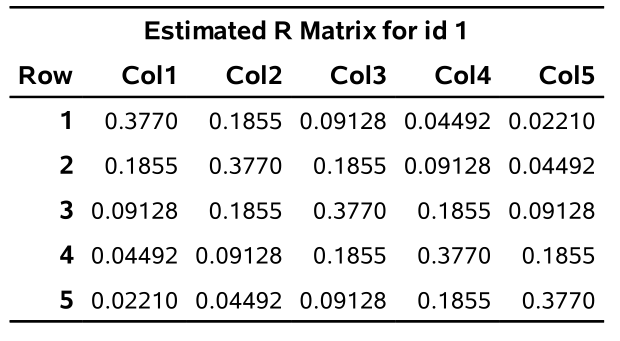
\includegraphics[width = 0.45\linewidth]{img/c5/slides6-e15a}
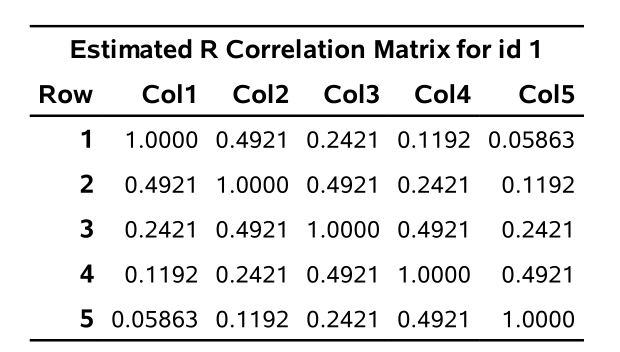
\includegraphics[width = 0.45\linewidth]{img/c5/slides6-e15b}
\end{center}
\bi
\item We can see that the correlation between two observations decreases the further apart they are in time. 
\item This is exactly what we want to model when choosing the  $\mathsf{AR}(1)$ covariance structure.
\ei
\end{frame}

\begin{frame}[fragile]
\frametitle{Parameters in the $\mathsf{AR}(1)$ covariance/correlation structure}
\begin{center}
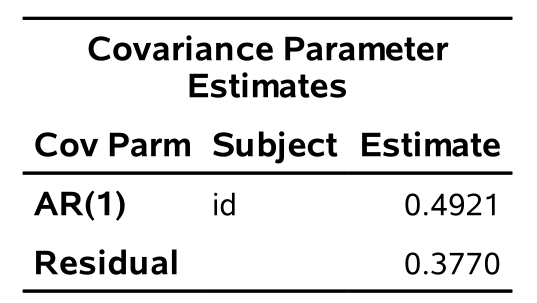
\includegraphics[width = 0.4\linewidth]{img/c5/slides6-e16}
\end{center}
\bi
\item We can see that the estimate of the parameter $\rho$ is $\hat{\rho} =0.492$.
% It's also significantly different from $0$ (negligible $p$-value).
\item We can verify in the correlation matrix for subject $1$ that the correlation between $t_1$ and $t_2$ is $0.492$ times the correlation between $t_1$ and $t_3$; that is, it is $0.492^2=0.24$
\item Note: in the compound symmetry model, the estimated correlation between two observations from the same person (regardless of the time between measures) was $0.356$.

\ei
\end{frame}



\begin{frame}[fragile]
\frametitle{Mean parameter estimates}
\begin{center}
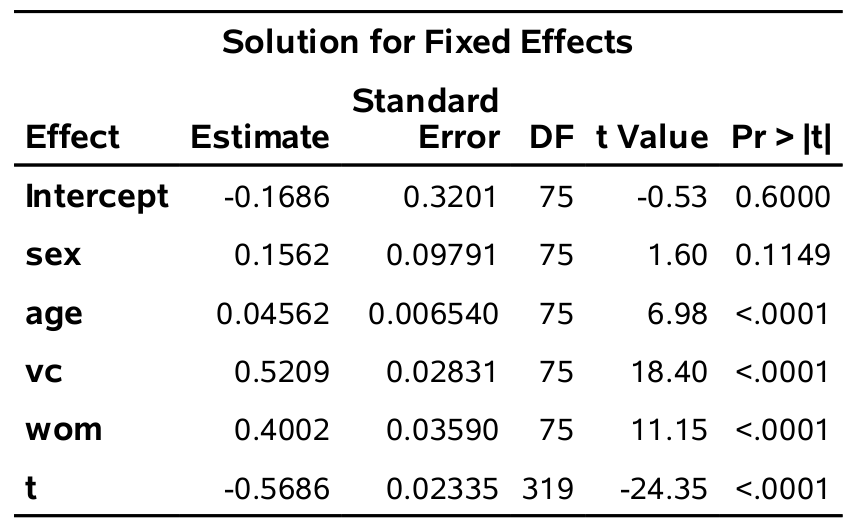
\includegraphics[width = 0.7\linewidth]{img/c5/slides6-e17}
\end{center}
\bi
\item The estimates of the $\beta$ parameters are very similar to those from the previous model (with the compound symmetry structure), but not identical. 
\item The explanatory variables are all significant except for \code{sex}. The conclusions are the same as those from the previous model.
\ei
\end{frame}

\end{document}
